\documentclass[12pt]{article}

% General
\usepackage[round]{natbib}
\usepackage{setspace}
\usepackage{geometry}
\usepackage[section]{placeins}
\usepackage[hidelinks]{hyperref}
\usepackage{graphicx}
\usepackage{xcolor}
\usepackage{titlesec}
\usepackage[page]{appendix}
\usepackage{enumerate}

% Tables/Figures
\usepackage{lscape}
\usepackage{booktabs}
\usepackage{rotating}
\usepackage{multirow}
\usepackage{longtable}
\usepackage{caption}
\usepackage{subcaption}
\usepackage{float}
\usepackage{tabularx}
\usepackage{ragged2e}
\newcolumntype{Y}{>{\RaggedRight\arraybackslash}X}
\usepackage{pdflscape}
\usepackage{afterpage}

% Math
\usepackage{amsmath}
\usepackage{amssymb}
\usepackage{amsthm}
\usepackage{mathtools}
\usepackage{dsfont}

\usepackage{tikz}
\usetikzlibrary{bayesnet}

% \doublespacing
\onehalfspacing
% \singlespacing

% \numberwithin{equation}{section}

\geometry{paper=letterpaper, margin=1in}
\captionsetup{font=small}

% Code
\usepackage{textcomp}
\usepackage{sourcecodepro}
\usepackage{listings}
\definecolor{commentgrey}{gray}{0.45}
\definecolor{backgray}{gray}{0.96}
\lstset{
  basicstyle=\footnotesize\ttfamily, keywordstyle=\footnotesize,
  backgroundcolor=\color{backgray}, commentstyle=\color{commentgrey},
  frame=single, rulecolor=\color{backgray}, showstringspaces=false,
  breakatwhitespace=true, breaklines=true, upquote=true,
  numbers=left, numberstyle=\footnotesize\color{commentgrey}}

%%%%%%%%%%%%%%%%%%%%%%%%%%%%%%%%%%%%%%%%%%%%%%%%%%%%%%%%%%%%%%%%%%%%%%%%%%%%%%
% User-defined LaTeX commands
\DeclareMathOperator{\Var}{Var}
\DeclareMathOperator{\Cov}{Cov}
\DeclareMathOperator{\Corr}{Corr}
\DeclareMathOperator*{\argmax}{arg\,max}
\DeclareMathOperator*{\argmin}{arg\,min}
\DeclarePairedDelimiter{\abs}{\lvert}{\rvert}
\DeclarePairedDelimiter{\norm}{\lVert}{\rVert}
\newcommand*{\expp}[1]{\exp\left(#1\right)}
\newcommand*{\foralls}{\ \forall \ }
\newcommand*{\st}{\text{ s.t. }}
\newcommand*{\E}{\mathbb E}
\newcommand*{\R}{\mathbb R}
\newcommand*{\I}{\mathds{1}}
\newcommand*{\Prob}{\mathbb P}
\newcommand*{\convas}[1]{\xrightarrow{#1}}
\newcommand*{\conv}{\convas{}}
\newcommand*{\cond}{\;\ifnum\currentgrouptype=16 \middle\fi|\;}
\newcommand*{\defeq}{%
  \mathrel{\overset{\makebox[0pt]{\mbox{\normalfont\tiny\sffamily def}}}{=}}}
\newcommand*{\notorth}{\ensuremath{\perp\!\!\!\!\!\!\diagup\!\!\!\!\!\!\perp}}
\newcommand*{\orth}{\ensuremath{\perp\!\!\!\perp}}
\newcommand*{\evalat}{\,\big\rvert}
\newcommand*{\dif}{\,d}
\newcommand*{\difto}[1]{\,d^#1}
\newcommand*{\difbot}[1]{\frac{d}{d#1}}
\newcommand*{\partialbot}[1]{\frac{\partial}{\partial#1}}
\newcommand*{\m}[1]{\textbf{#1}}
\newcommand*{\bmath}[1]{\boldsymbol{#1}}

\newcommand*{\yestag}{\addtocounter{equation}{1}\tag{\theequation}}
\newcommand*{\notaligned}[1]{\noalign{$\displaystyle #1$}}
\newcommand*{\ttilde}{{\raise.17ex\hbox{$\scriptstyle\sim$}}}

\makeatletter
\newsavebox{\mybox}\newsavebox{\mysim}
\newcommand*{\distas}[1]{%
  \savebox{\mybox}{\hbox{\kern3pt$\scriptstyle#1$\kern3pt}}%
  \savebox{\mysim}{\hbox{$\sim$}}%
  \mathbin{\overset{#1}{\kern\z@\resizebox{\wd\mybox}{\ht\mysim}{$\sim$}}}%
}
\makeatother
\newcommand*{\dist}{\sim}
\newcommand*{\distiid}{\distas{\text{i.i.d}}}

\makeatletter
\def\moverlay{\mathpalette\mov@rlay}
\def\mov@rlay#1#2{\leavevmode\vtop{%
   \baselineskip\z@skip \lineskiplimit-\maxdimen
   \ialign{\hfil$\m@th#1##$\hfil\cr#2\crcr}}}
\newcommand*{\charfusion}[3][\mathord]{
  #1{\ifx#1\mathop\vphantom{#2}\fi\mathpalette\mov@rlay{#2\cr#3}}
  \ifx#1\mathop\expandafter\displaylimits\fi}
\makeatother
\newcommand*{\cupdot}{\charfusion[\mathbin]{\cup}{\cdot}}
\newcommand*{\bigcupdot}{\charfusion[\mathop]{\bigcup}{\cdot}}

\newcommand*{\mt}[1]{\text{\normalfont #1}}

\newtheorem{theorem}{Theorem}[section]
\newtheorem{theorem*}{Theorem}
\newtheorem{corollary}{Corollary}[section]
\newtheorem{proposition}{Proposition}[section]
\newtheorem{lemma}{Lemma}[section]

\theoremstyle{definition}
\newtheorem{definition}{Definition}[section]
\newtheorem{definition*}{Definition}
\newtheorem{example}{Example}[section]
\newtheorem*{properties}{Properties}

\newtheoremstyle{algodesc}{}{}{}{}{\bfseries}{.}{ }{}%
\theoremstyle{algodesc}
\newtheorem{algodesc}{Algorithm}
%%%%%%%%%%%%%%%%%%%%%%%%%%%%%%%%%%%%%%%%%%%%%%%%%%%%%%%%%%%%%%%%%%%%%%%%%%%%%%


\begin{document}

\title{Taxi Trip Density Estimation in NYC\thanks{2016 Applied Statistics Qualifying Exam report.}}
\author{
    Roger Fan\footnote{\url{rogerfan@umich.edu}}
}
\date{May 26, 2016}

\maketitle


\section{Introduction}
Demand estimation is a crucial problem for taxicab companies (and potentially other ride-share services), allowing them to more effectively plan and adjust deployments. Using a dataset of New York City taxi trip data, I will show how clustering and density estimation techniques can be applied to this problem. Although taxi trip originations are not perfect indicators of demand, as a completed trip requires both the demand for a trip and a taxi available to supply it, I will use taxi origination locations to hopefully proxy for actual taxi demand.

I use a Gaussian mixture model (GMM) to estimate the density of trip origination locations in New York City. This method allows us to effectively condense the information from data on millions of taxi trip originations to a finite number of Gaussian distributions over the city.

However, I expect that the demand for taxis would change over time, a factor that would be vital to most applications of this analysis. To better handle this issue, I design a extension to the standard Gaussian mixture model that allows for time-varying mixing weights and an Expectation-Maximization (EM) algorithm to estimate it.


\section{Data}
The NYC Taxi and Limousine Commision (TLC) provides extensive data on taxicab trips in New York City for the last several years.\footnote{Available at \url{http://www.nyc.gov/html/tlc/html/about/trip_record_data.shtml}.} This data includes both yellow cabs, which primarily pick up street hails in Manhattan and at the airports, and green cabs, which can only be hailed in northern Manhattan and the outer boroughs.

The primary variables of interest are the time and location of each trip's pickup and dropoff. Location data is encoded as latitude and longitude, which we will be able to use directly, and time data is recorded to the second, though we will primarily be using data at the hourly frequency in this analysis.

To simplify estimation and computation, we will focus on taxi rides conducted during a single week, December 7-10, 2015. We omit Friday-Sunday of the week to avoid complicating the analysis with weekend data, and so are left with four days of weekday data, consisting of just over 1.7 million individual taxi rides. Of these, around 25 thousand are missing location data, which is a small enough number that it is safe to simply omit them. And finally, there are around 100 outlier trips that have nonsensical or extreme pickup or dropoff locations that are omitted, leaving a final dataset of 1,688,673 taxi trips.


\section{Density Estimation}
We can consider taxi demand as a density estimation problem, where each trip's origination location is a draw from the underlying density. Estimating taxi demand then simply becomes a problem of estimating the underlying (2-dimensional) density of taxi originations.

\subsection{Gaussian Mixture Model} \label{sec:gmm}
In order to estimate the density, we will assume that joint density for $X$ comes from a $J$-component Gaussian mixture model and estimate the model using the EM algorithm, which has been standard since \citet{dempsterlairdrubin77} first introduced the EM algorithm. We introduce a latent variable $Z$ that indicates group membership and have a generative model defined by
\begin{equation} \label{eq:gmm}
\begin{aligned}
Z &\dist \mt{Categorical}(\pi_1, \dots, \pi_J) \\
X \cond Z = j &\dist \mt{Gaussian}(\mu_j, \Sigma_j)
\end{aligned}
\end{equation}
The EM algorithm updates are therefore as follows.
\begin{enumerate}
\item
  E-step: Estimate the group probabilities $p_{ij}^{(t+1)}$ conditional on the current parameter estimates.
  \begin{equation} \label{eq:gmm_estep}
  p_{ij}^{(t+1)} = \frac{\pi_j^{(t)} P( X_i \cond \mu_j^{(t)}, \Sigma_j^{(t)})}{\sum_{j'=1}^J \pi_{j'}^{(t)} P( X_i \cond \mu_{j'}^{(t)}, \Sigma_{j'}^{(t)})}
  \end{equation}

\item
  M-step: Estimate the parameters using maximum likelihood estimators conditional on the group probability estimates.
  \begin{equation} \label{eq:gmm_mstep}
  \begin{aligned}
  \pi_j^{(t+1)} &= \frac{1}{n} \sum_{i=1}^n p_{ij}^{(t+1)} \\
  \mu_j^{(t+1)} &= \frac{\sum_{i=1}^n p_{ij}^{(t+1)} X_i}{\sum_{i=1}^n p_{ij}^{(t+1)}} \\
  \Sigma_j^{(t+1)} &= \frac{\sum_{i=1}^n p_{ij}^{(t+1)} (X_i - \mu_j^{(t+1)}) (X_i - \mu_j^{(t+1)})^T}{\sum_{i=1}^n p_{ij}^{(t+1)}}
  \end{aligned}
  \end{equation}
\end{enumerate}

\subsection{Time-Varying Mixing Components}
However, the model described in Equation~\ref{eq:gmm} has a major weakness: it does not incorporate time information. We would expect that the demand for taxis may vary significantly over different time periods. To illustrate this, Figure~\ref{fig:diff} plots taxi originations for two time periods, 7am-9am and 10am-12am.\footnote{These subsamples have approximately the same number of observations.} Even using just the raw data, we can identify several areas that exhibit differences. In particular, the morning taxi demand seems to be higher in southwest Brooklyn (-74.00, 40.68), nothern Queens (-73.92, 40.76), the Bronx (-73.90, 40.82), and nothern Manhattan (-73.95, 40.81), while nighttime demand is higher in Williamsburg in northern Brooklyn (-73.94, 40.71). The morning periods in particular are as we might expect, communities that commute into the city during morning rush hour.

\begin{figure}[htbp] \centering
  \begin{subfigure}[t]{.49\linewidth}
    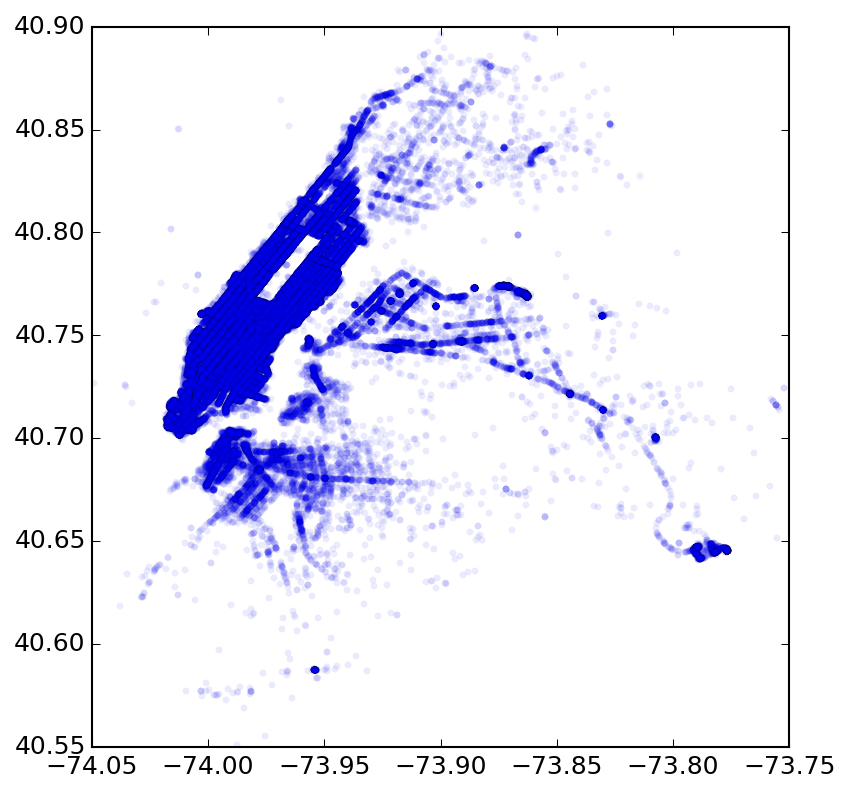
\includegraphics[width=\linewidth]{./include/diff_morningrush.png}
    \caption{7am-9am} \label{fig:diff:morning}
  \end{subfigure}
  \begin{subfigure}[t]{.49\linewidth}
    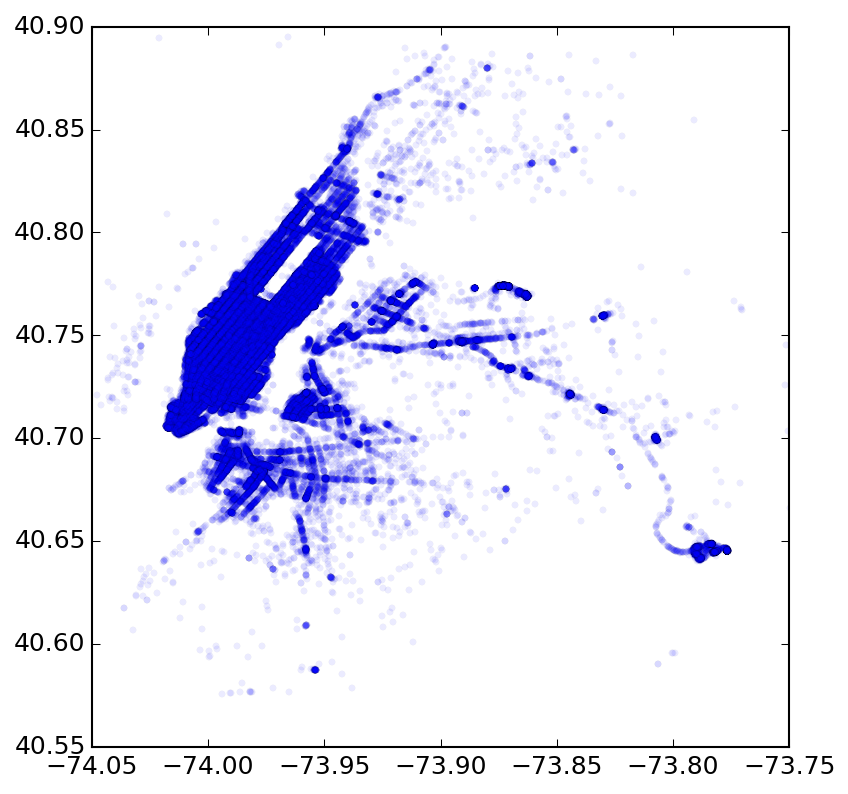
\includegraphics[width=\linewidth]{./include/diff_night.png}
    \caption{10pm-12am} \label{fig:diff:night}
  \end{subfigure}
  \caption{Taxi originations during morning rush hour (7am-9am) and at night (10pm-12am).}
  \label{fig:diff}
\end{figure}

This motivates an extension to the Gaussian mixture model that can incorporate time-varying information. We will assume that the component distributions are the same over time, as it seems reasonable to assume that the location and shape of each cluster is constant. But we will allow the mixing proportions to vary between time periods, allowing the demand from each neighborhood to shift over different time periods. This, for instance, allows for phenomenon such as commuter neighborhoods that have high demand during rush hour but little during the day. It will also hopefully allow us to identify clusters that are only visible during specific time periods.

To account for this, we incorporate an additional variable $Y \in \{1, \dots, K\}$ to track the time period of the obervation $X$. We will assume that $Y$ is fixed and exogenous. Then our model becomes
\begin{equation} \label{eq:gmm_cat}
\begin{aligned}
Z \cond Y = k &\dist \mt{Categorical}(\pi_{k1}, \dots, \pi_{kJ}) \\
X \cond Z = j &\dist \mt{Gaussian}(\mu_j, \Sigma_j)
\end{aligned}
\end{equation}
The EM algorithm is similar to the one described in Section~\ref{sec:gmm}, replacing the group probability update in Equation~\ref{eq:gmm_estep} with
\begin{equation} \label{eq:gmm_cat_estep}
p_{ij}^{(t+1)} = \frac{\pi_{Y_i j}^{(t)} P( X_i \cond \mu_j^{(t)}, \Sigma_j^{(t)})}{\sum_{j'=1}^J \pi_{Y_i j'}^{(t)} P( X_i \cond \mu_{j'}^{(t)}, \Sigma_{j'}^{(t)})}
\end{equation}
And replacing the mixing component update in Equation~\ref{eq:gmm_mstep} with
\begin{equation} \label{eq:gmm_cat_mstep}
\pi_{kj}^{(t+1)} = \frac{\sum_{i=1}^n \I(Y_i = k) p_{ij}^{(t+1)} }{\sum_{i=1}^n \I(Y_i = k)}
\end{equation}

Note that the advantage of dividing time into a (small) number of categories and estimating each category's mixing components separately is that it does not add much computational complexity over the standard GMM model. A richer model might be to assume the mixing proportion for each cluster varies smoothly over time and then use a local averaging or kernel regression method instead of Equation~\ref{eq:gmm_cat_mstep}, but this would add a significant computational burden.


\section{Results}
Figure~\ref{fig:gmm_res} shows the estimated cluster centers and density of the basic GMM model, described in Equation~\ref{eq:gmm}. We can see that the contours of the estimated density visually correspond well to the raw origination data. Several of the important features of NYC are identifiable, including the overall shape and size of the outer boroughs, the locations of JFK and LaGuardia airports (the two hotspots to the east), and the overall shape of Manhattan and Midtown, including a cool spot in Central Park. The red centers indicate the three clusters with the highest estimated mixing proportions, which together make up around 37\% of originations.

\begin{figure}[tb] \centering
  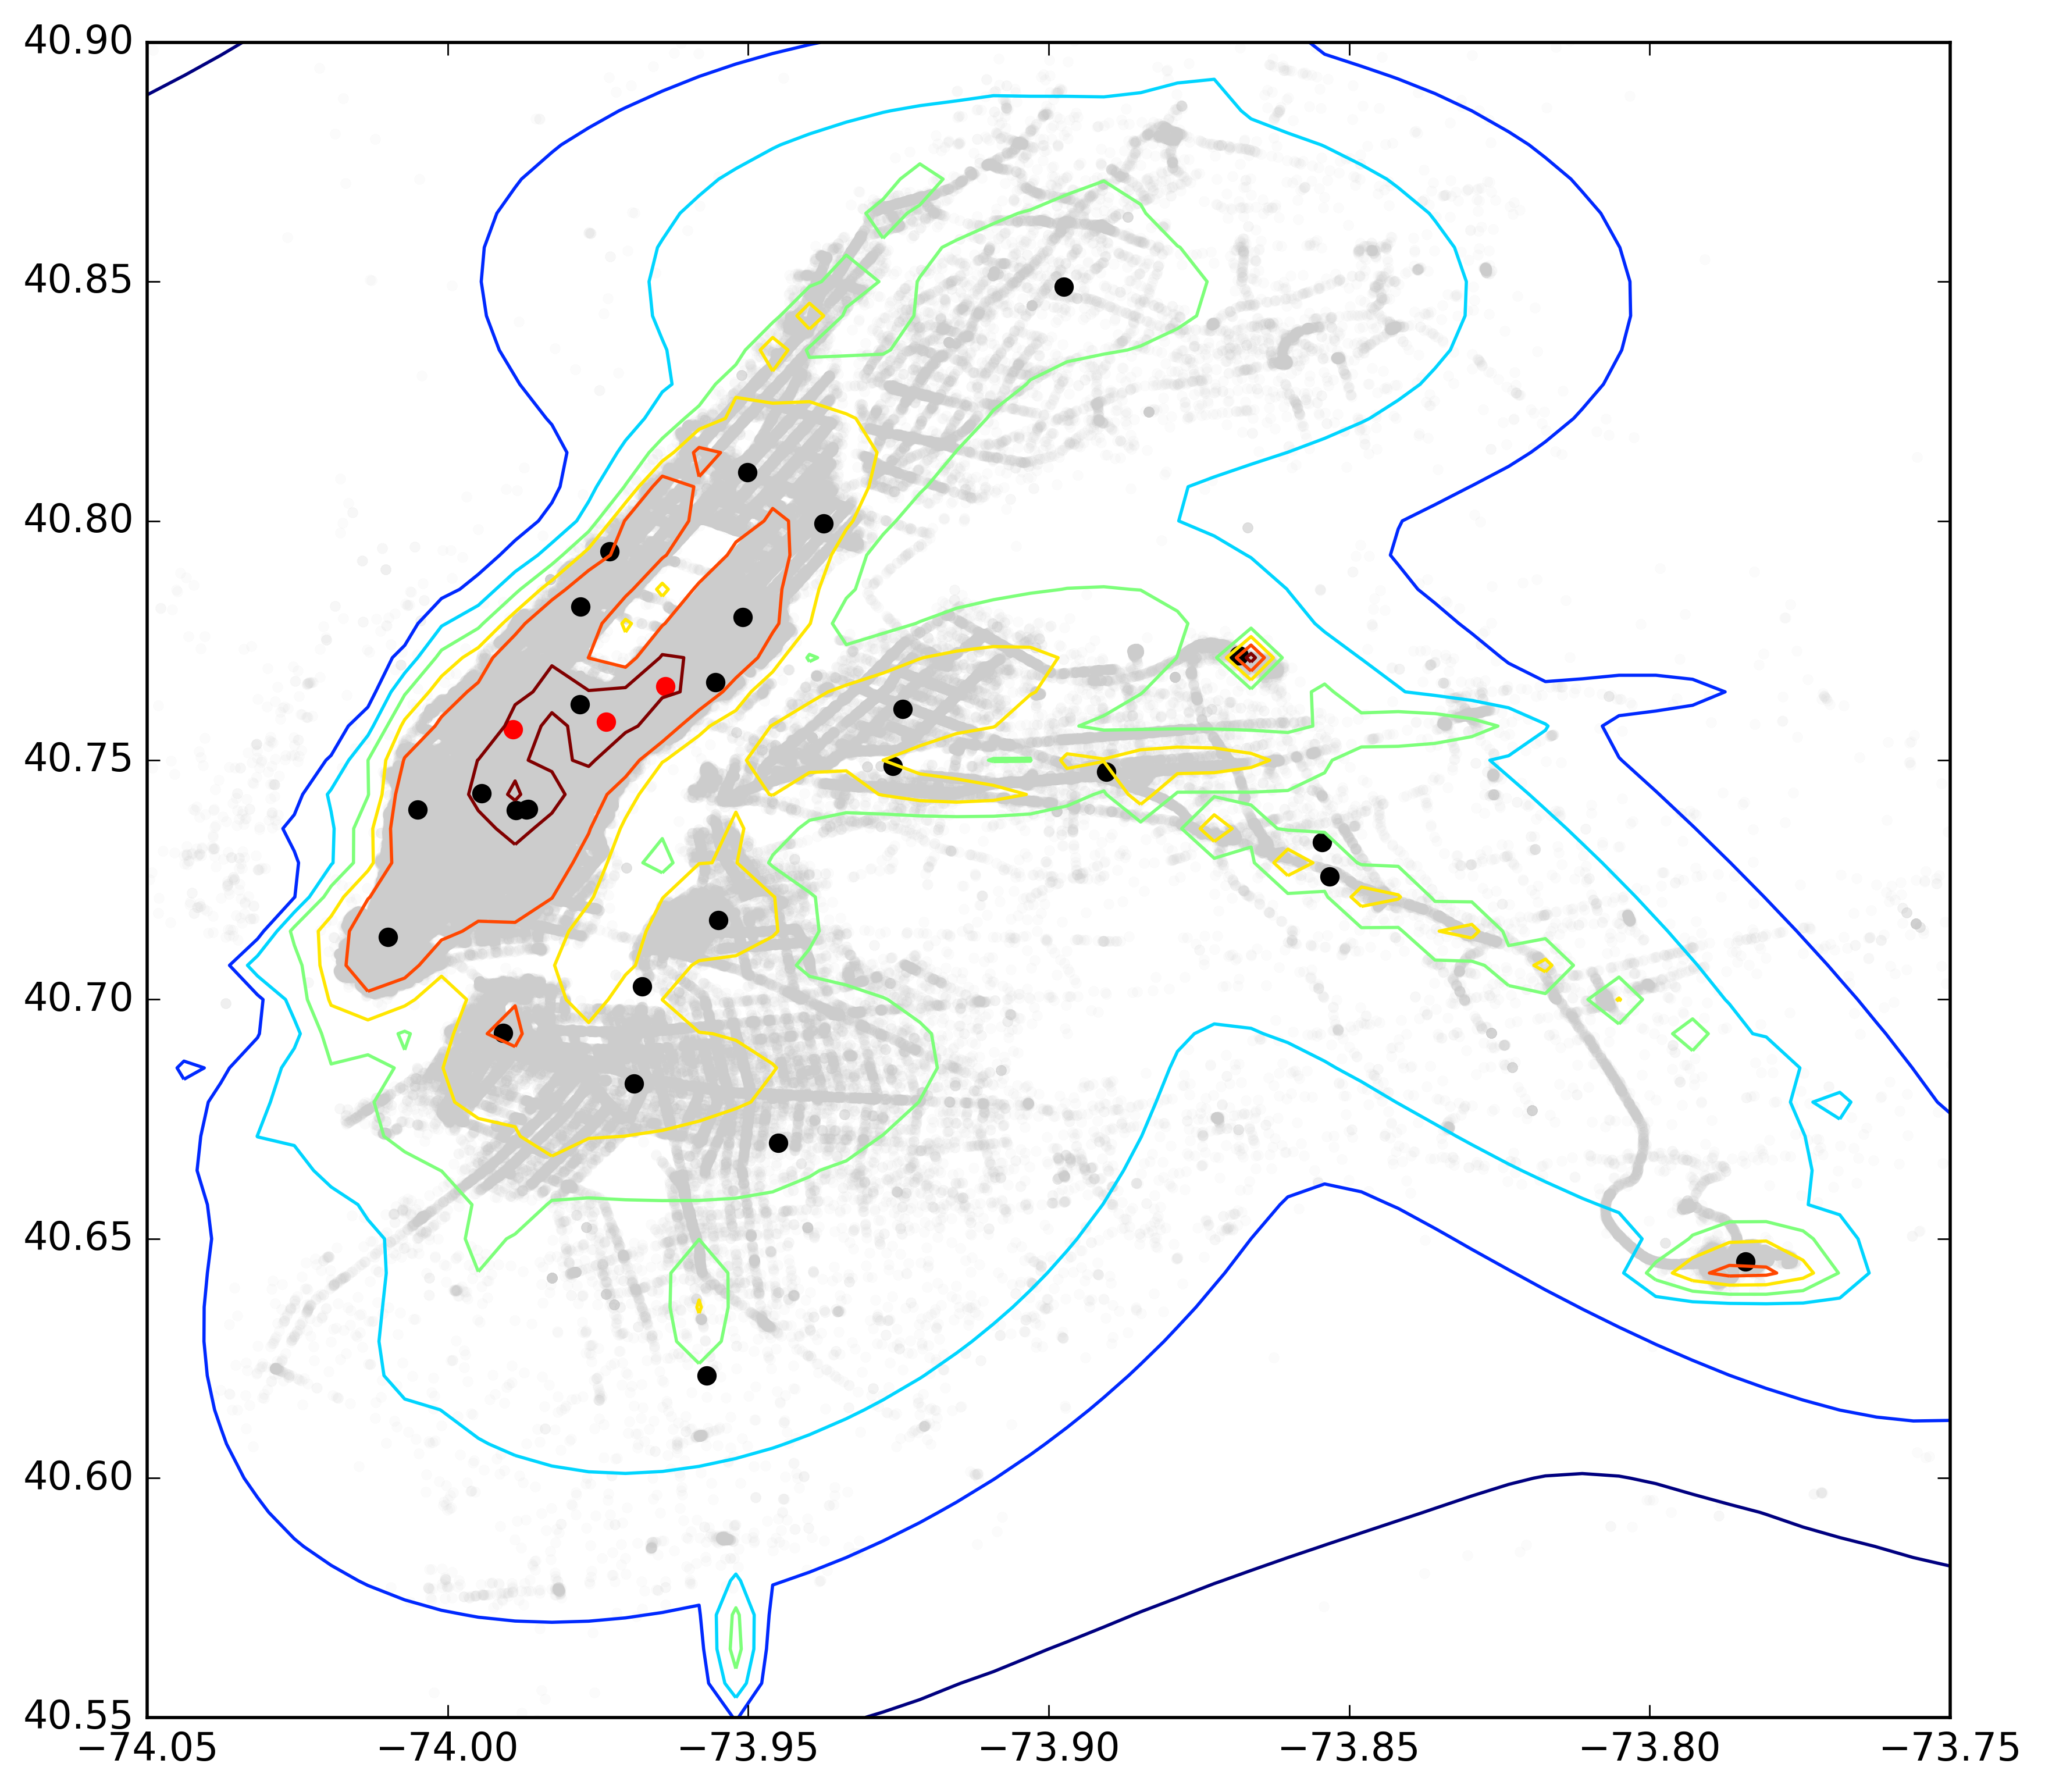
\includegraphics[width=0.8\linewidth]{./include/gmm_res.png}
  \caption{Estimated cluster centers and density of NYC taxi originations using a Gaussian mixture model.}
  \label{fig:gmm_res}
\end{figure}

To estimate the GMM model with time-varying mixing proportions described in Equation~\ref{eq:gmm_cat}, we first need to divide time into six categories. Attempting to adhere to common-sense work day divisions, I propose using early morning (2am-7am), morning rush hour (7am-9am), work day (9am-4pm), evening rush hour (4pm-6pm), evening (6pm-10pm), and night (10pm-2am). Figure~\ref{fig:time} shows the frequency of taxi pickups over time as well as these proposed categories. We can see that the categories seem to correspond well to natural divisions in data, with boundaries roughly tracking change points in the histogram.

\begin{figure}[htb] \centering
  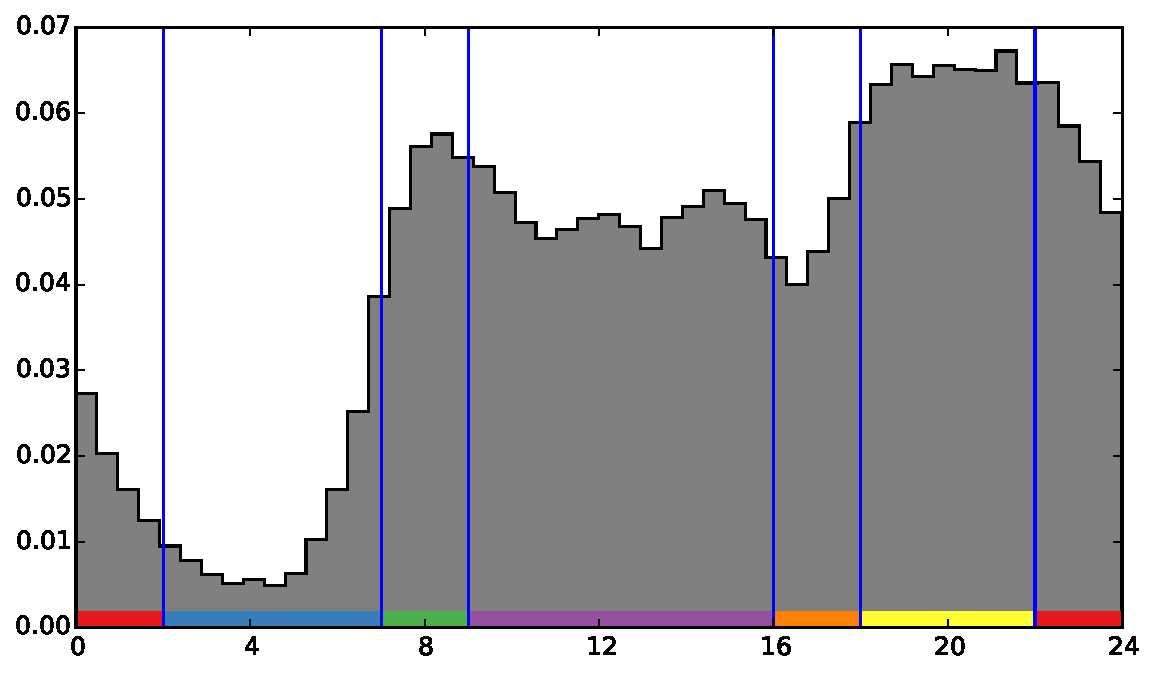
\includegraphics[width=0.8\linewidth]{./include/time.pdf}
  \caption{Taxi pickups over time with proposed time categories.}
  \label{fig:time}
\end{figure}

Figure~\ref{fig:gmm_cat_res} shows the estimated centers for this model. We can see that the centers outside of Manhattan are nearly identical to those in Figure~\ref{fig:gmm_res}, but that the centers inside Manhattan are a little more evenly distributed.

\begin{figure}[tb] \centering
  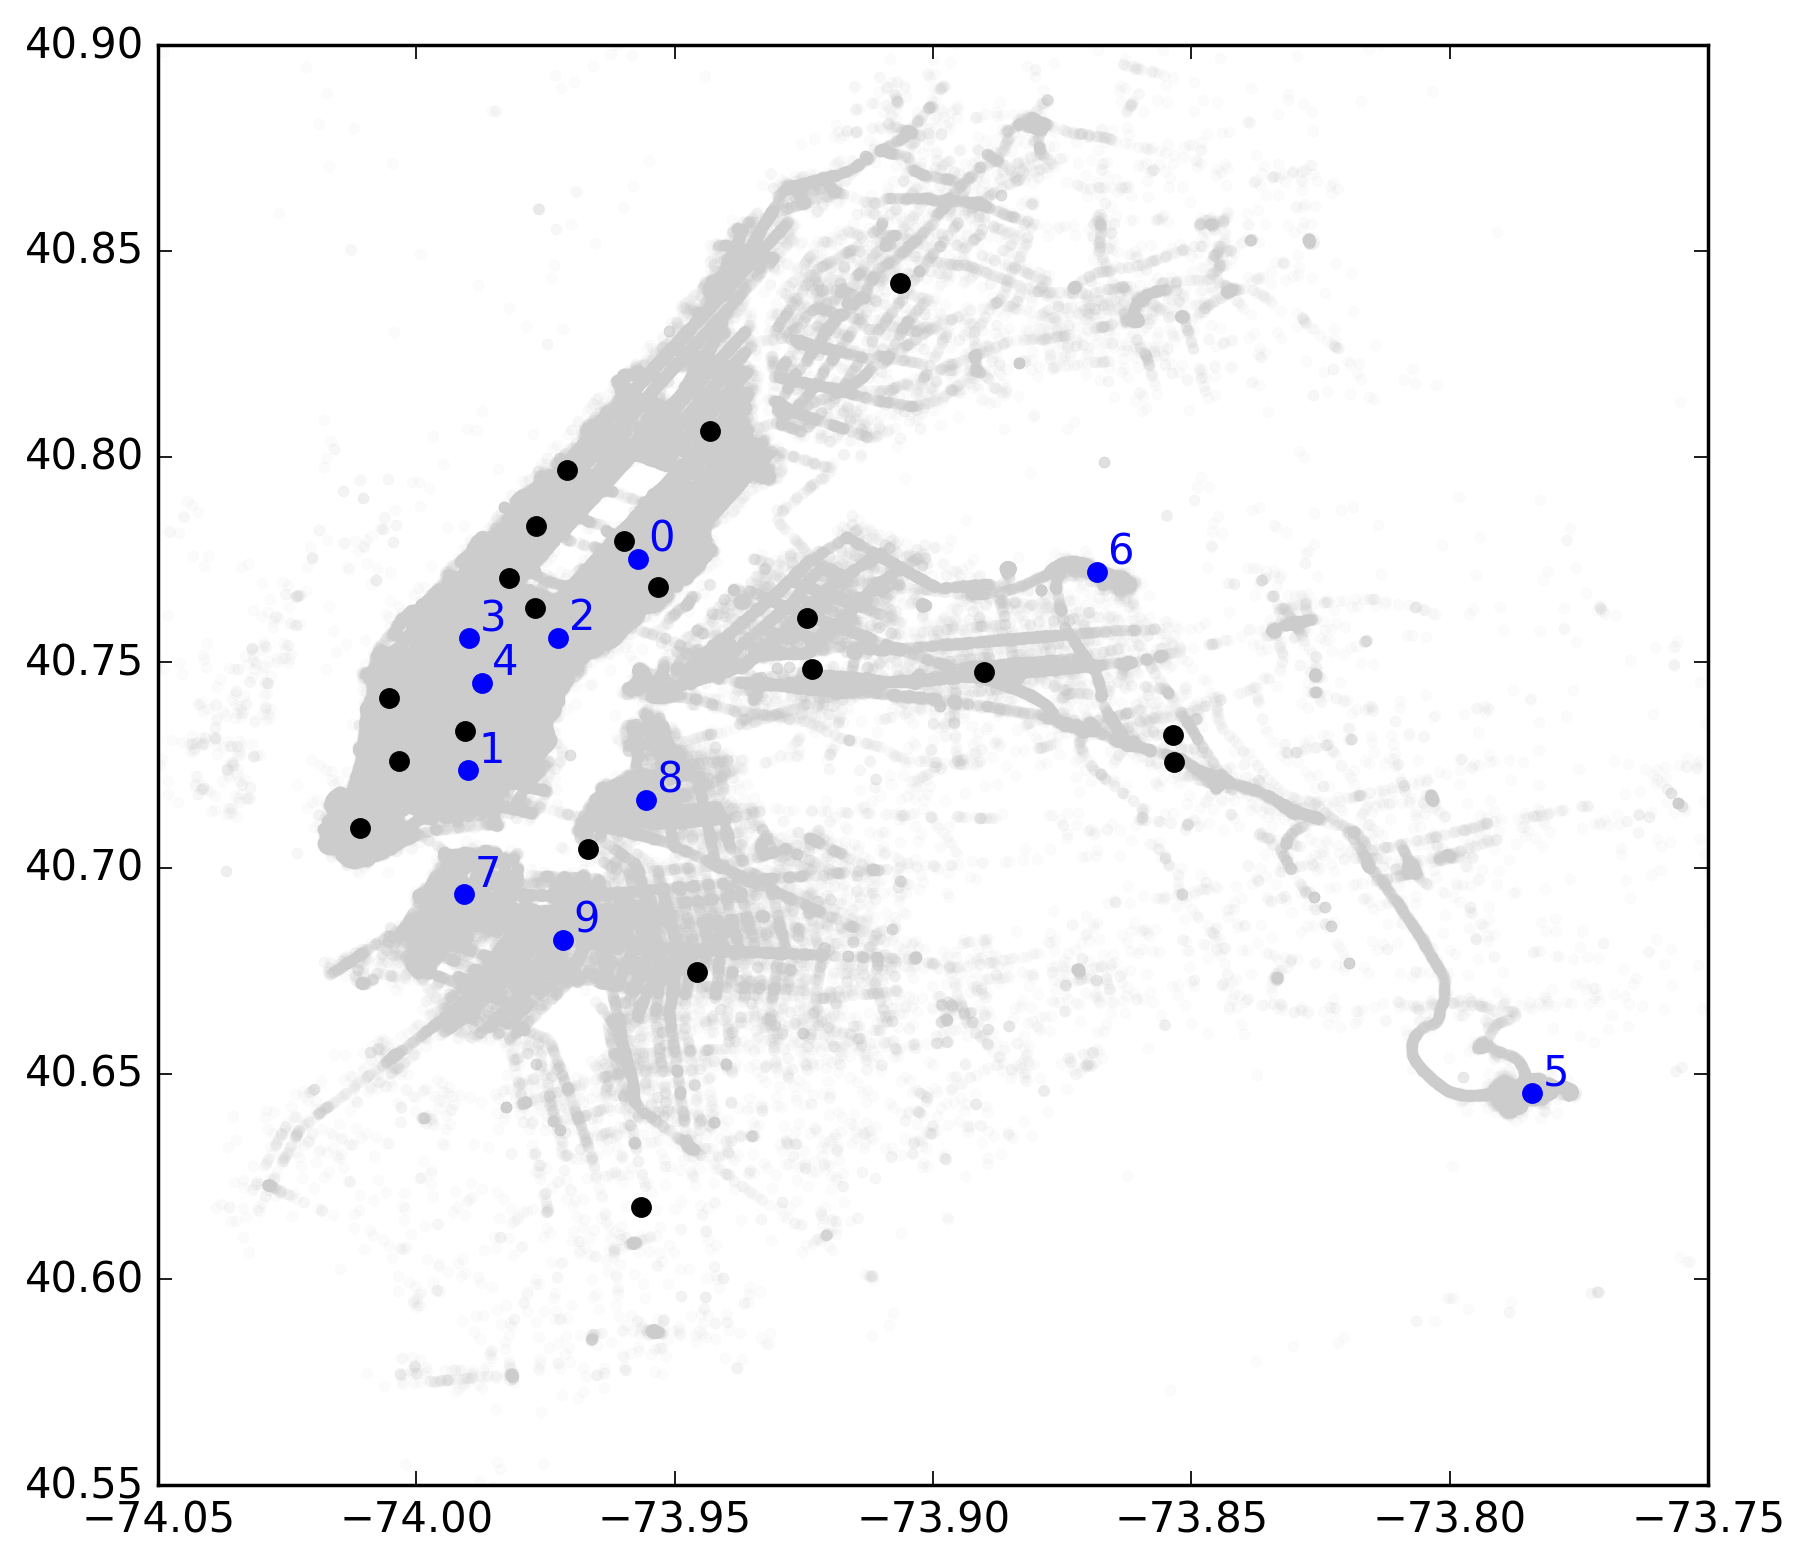
\includegraphics[width=0.7\linewidth]{./include/gmm_cat_res.png}
  \caption{Estimated cluster centers of NYC taxi originations using a Gaussian mixture model with time-varying mixing proportions.}
  \label{fig:gmm_cat_res}
\end{figure}

Table~\ref{tab:mixing} shows the evolution of mixing proportions for a subset of the clusters. We can see that there is significant variation across time for many of the clusters, and that the patterns can also be very different. JFK (cluster 5) and LaGuardia (cluster 6) have similar patterns over time except for in the early morning, where JFK has a relatively high percentage of taxi originations and LaGuardia has almost none. Or consider southwest Brooklyn (cluster 7), which is primarily busy during rush hour and the work day, compared to Williamsburg (cluster 8), which has more originations at night and in the early morning and very few during the day. Clusters in Mahattan can also be very different, as East Village/Lower East Side (cluster 1) seems to be a night-life area, while the Upper East Side (cluster 0) has relatively few originations at night.

\begin{table}[htb] \centering
\begin{tabular}{rrrrrrrrrrr}
  \toprule
   & \multicolumn{5}{c}{Manhattan} & \multicolumn{2}{c}{Airports} & \multicolumn{3}{c}{Boroughs} \\
   \cmidrule(lr){2-6} \cmidrule(lr){7-8} \cmidrule(lr){9-11}
   & \multicolumn{1}{c}{0} & \multicolumn{1}{c}{1} & \multicolumn{1}{c}{2} & \multicolumn{1}{c}{3} & \multicolumn{1}{c}{4} & \multicolumn{1}{c}{5} & \multicolumn{1}{c}{6} & \multicolumn{1}{c}{7} & \multicolumn{1}{c}{8} & \multicolumn{1}{c}{9} \\
  \midrule
  02:00-07:00 &  8.10 &  5.72 &  8.97 & 14.38 & 17.72 &  2.09 &  0.16 &  1.18 &  1.45 &  1.62 \\
  07:00-09:00 &  8.53 &  1.82 & 11.91 &  8.56 & 18.40 &  1.27 &  1.87 &  1.86 &  0.23 &  1.58 \\
  09:00-16:00 &  7.19 &  1.83 & 11.95 &  6.77 & 18.91 &  1.72 &  3.58 &  1.20 &  0.25 &  1.23  \\
  16:00-18:00 &  8.06 &  1.68 &  9.86 &  5.64 & 15.20 &  2.64 &  3.73 &  1.54 &  0.36 &  1.59 \\
  18:00-22:00 &  6.78 &  3.76 & 12.51 &  7.14 & 17.64 &  1.75 &  2.54 &  1.30 &  0.73 &  1.71 \\
  22:00-02:00 &  4.19 &  8.61 & 12.23 &  8.55 & 18.02 &  1.69 &  1.96 &  0.97 &  2.04 &  1.92 \\
  \bottomrule
\end{tabular}
\caption{Estimated mixing proportions for a subset of clusters.}
\label{tab:mixing}
\end{table}

Figure~\ref{fig:dist} compares the estimated distributions for morning rush hour and late-night. We can see that many of the same patterns visible in Figure~\ref{fig:diff} are also clear here, where the northern and southern boroughs have more originations in the morning while Williamsburg has more originations at night. But using the estimated distributions, we can also identify patterns in Manhattan that were impossible to see with the raw data. For instance, we can clearly see the nighttime hotspot in southern Manhattan that is the Lower East Side, and we can see how northern Manhattan and the Upper East Side have fewer night originations.

\begin{figure}[htbp] \centering
  \begin{subfigure}[t]{.49\linewidth}
    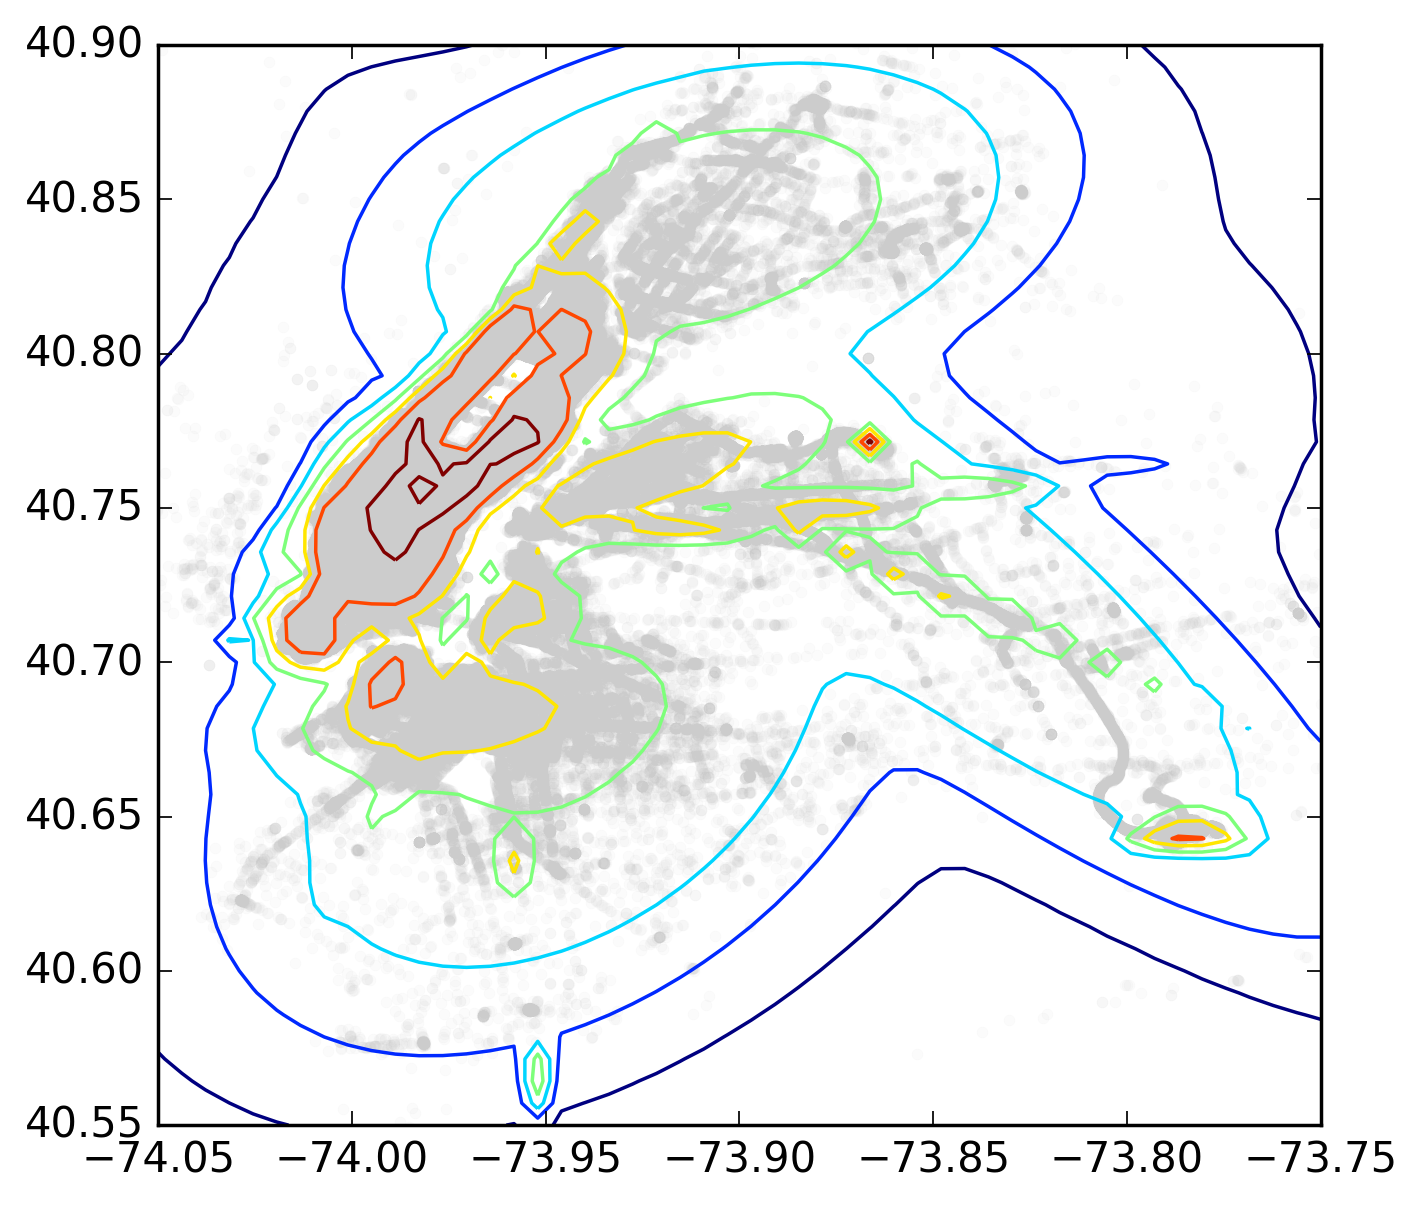
\includegraphics[width=\linewidth]{./include/gmm_cat_morn.png}
    \caption{7am-9am} \label{fig:dist:morning}
  \end{subfigure}
  \begin{subfigure}[t]{.49\linewidth}
    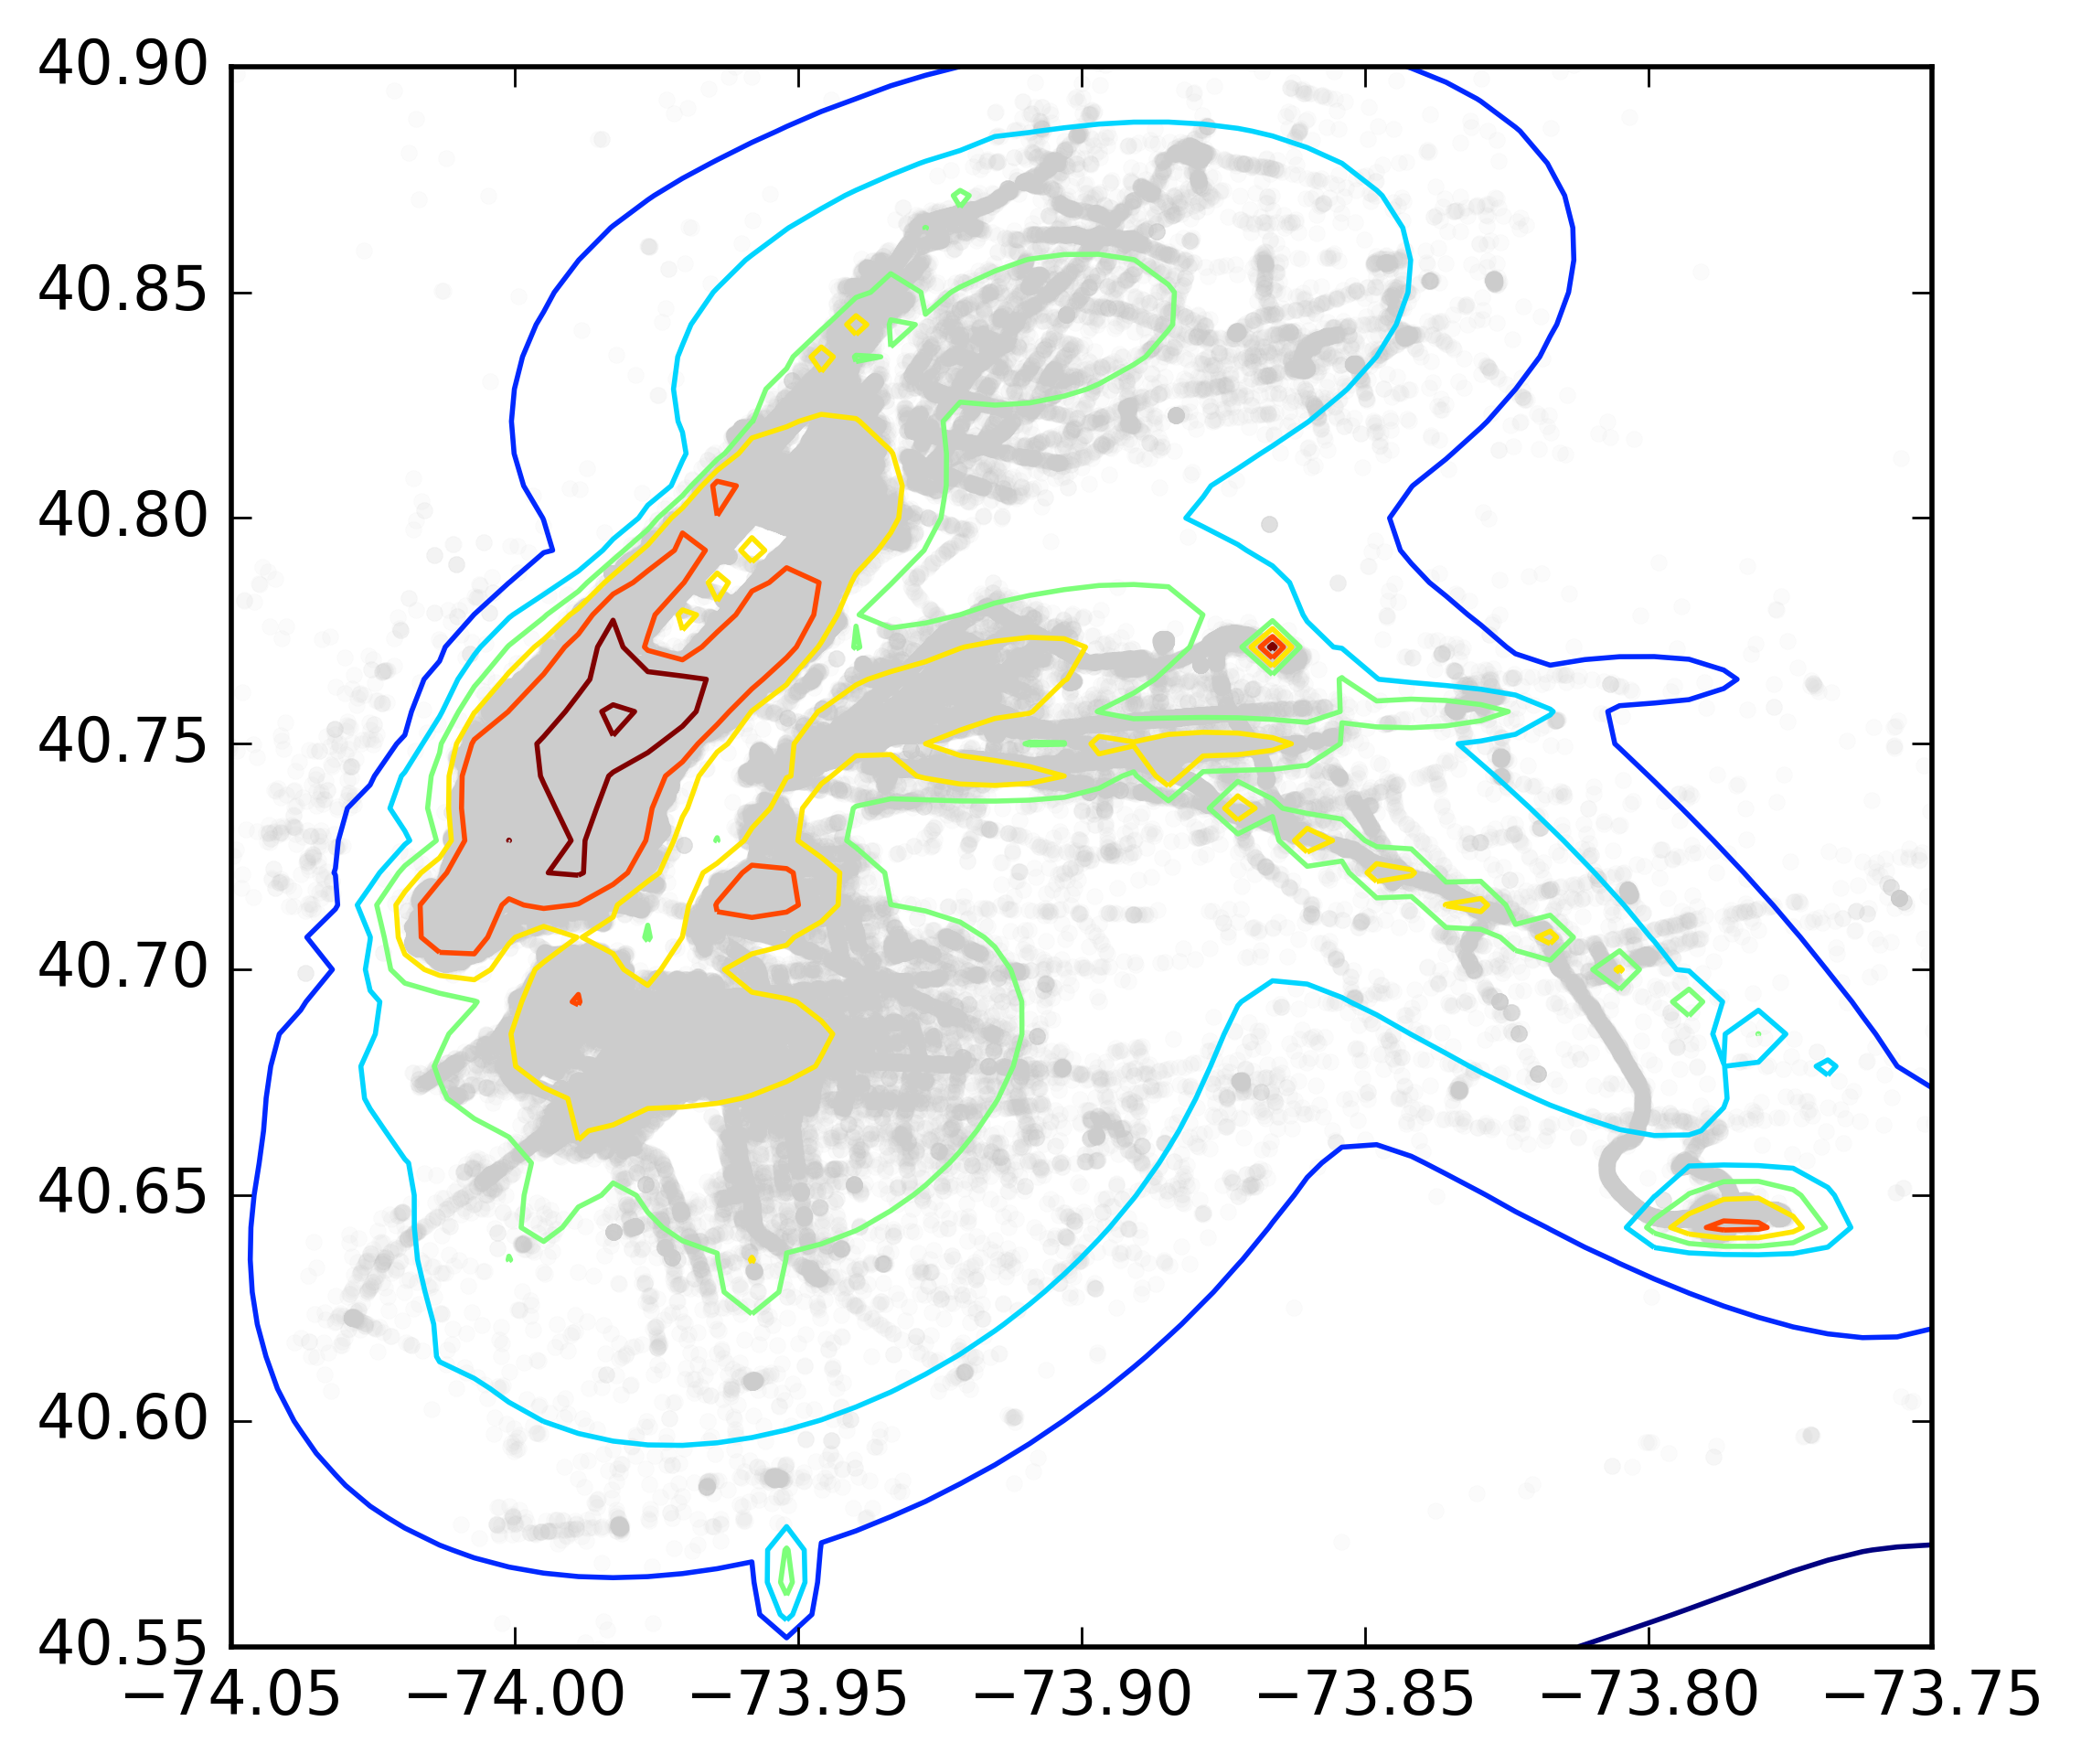
\includegraphics[width=\linewidth]{./include/gmm_cat_night.png}
    \caption{10pm-2am} \label{fig:dist:night}
  \end{subfigure}
  \begin{subfigure}[t]{.49\linewidth}
    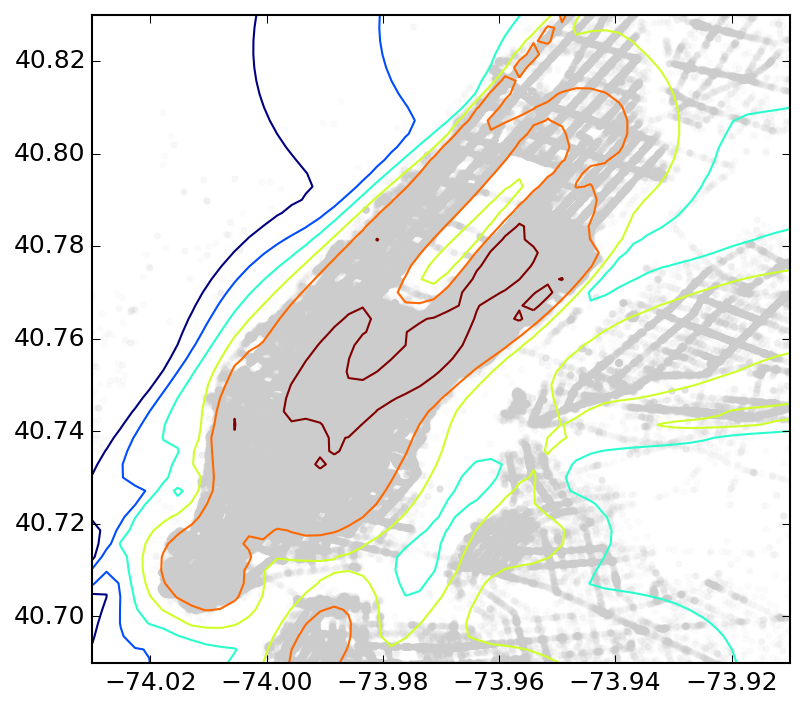
\includegraphics[width=\linewidth]{./include/gmm_cat_morn2.png}
    \caption{7am-9am} \label{fig:dist:morning2}
  \end{subfigure}
  \begin{subfigure}[t]{.49\linewidth}
    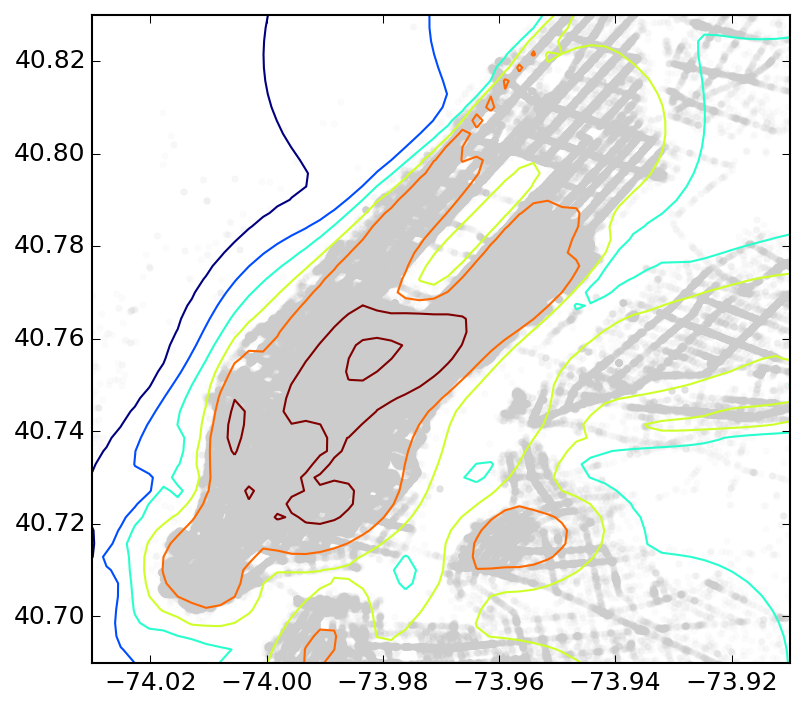
\includegraphics[width=\linewidth]{./include/gmm_cat_night2.png}
    \caption{10pm-2am} \label{fig:dist:night2}
  \end{subfigure}
  \caption{Some caption.}
  \label{fig:dist}
\end{figure}


\begin{table}[htb] \centering
\begin{tabular}{rrrr}
  \toprule
   & \multicolumn{1}{c}{GMM} & \multicolumn{1}{c}{ssGMM} & \multicolumn{1}{c}{tvGMM} \\
  \midrule
  02:00-07:00 &  125126 &  \textbf{128015} &  127873 \\
  07:00-09:00 &  235173 &  236006 &  \textbf{237738} \\
  09:00-16:00 &  773825 &  769287 &  \textbf{780562} \\
  16:00-18:00 &  211914 &  210956 &  \textbf{214326} \\
  18:00-22:00 &  601819 &  600960 &  \textbf{606997} \\
  22:00-02:00 &  292844 &  296174 &  \textbf{298605} \\
  \midrule
  Total       & 2240702 & 2241399 & \textbf{2266101} \\
  \bottomrule
\end{tabular}
\caption{Out-of-sample log-likelihoods.}
\label{tab:logliks}
\end{table}





\section{Conclusion}


\bibliographystyle{apa}
\bibliography{biblio}


\end{document}
